%# -*- coding: utf-8-unix -*-
%%==================================================
\chapter{B+-树}
\label{chap6}
\begin{itemize}[noitemsep,topsep=0pt,parsep=0pt,partopsep=0pt]
	\item 知识点:讲解相关知识点。
	\item 题型:直接上真题。
\end{itemize}

\section{知识点和方法论}

\subsection{知识点}
\begin{itemize}[noitemsep,topsep=0pt,parsep=0pt,partopsep=0pt]
	\item B树就是二叉搜索树
	\item B-树多路搜索树m阶
	\begin{itemize}[noitemsep,topsep=0pt,parsep=0pt,partopsep=0pt]
			\item 即平衡m叉查找树
			\item 要求所有的叶节点在同一层
			\item 每个节点最多有m个分支,
			\item 每个节点的关键字个数的范围 $\left \lceil m/2 \right \rceil -1  \le n \le m-1 $
			\item 根节点的关键字个数     1<= n <=m-1 
			\item 根节点最少有2个分支
			\item 非根非叶节点最少有 $\left \lceil m/2 \right \rceil$  分支,比如三阶节点最少有2个分支
			\item B 树的叶节点数 = 是所有非叶结点个数+1
	\end{itemize}
	\item 2-3 B-树 其每个非叶节点都有两个或三个子女,而且所有叶都在统一层上
	\item B+ 树
	\begin{itemize}[noitemsep,topsep=0pt,parsep=0pt,partopsep=0pt]
		\item n个关键字的节点有n个分支
		\item 每个节点的关键字的个数 n 的取值范围    向上取整(m/2) <= n <=m
        \item 根节点的关键字个数取值范围为2 <= n <=m,
	\end{itemize}
\end{itemize}
\subsection{方法论}
\begin{itemize}[noitemsep,topsep=0pt,parsep=0pt,partopsep=0pt]
	\item B-插入节点
	\begin{itemize}[noitemsep,topsep=0pt,parsep=0pt,partopsep=0pt]
	    \item 求节点中关键字个数的范围  3阶  1 ~ 2
		\item 中间一个节点上升即可,递归上升; 比如 有三个节点中间的节点上升
	\end{itemize}
	\item B-树删除操作
	\begin{itemize}[noitemsep,topsep=0pt,parsep=0pt,partopsep=0pt]
			\item 如果终端节点 > [向上取整(m/2)-1],可以直接删除
			\item 	如果终端节点数 = [向上取整(m/2)-1],但是左右兄弟中节点会> [向上取整(m/2)-1],向兄弟借节点,就像流水一样,或者叫队列
			\begin{figure}[H]
				\centering  % 环境中的内容居中排版
				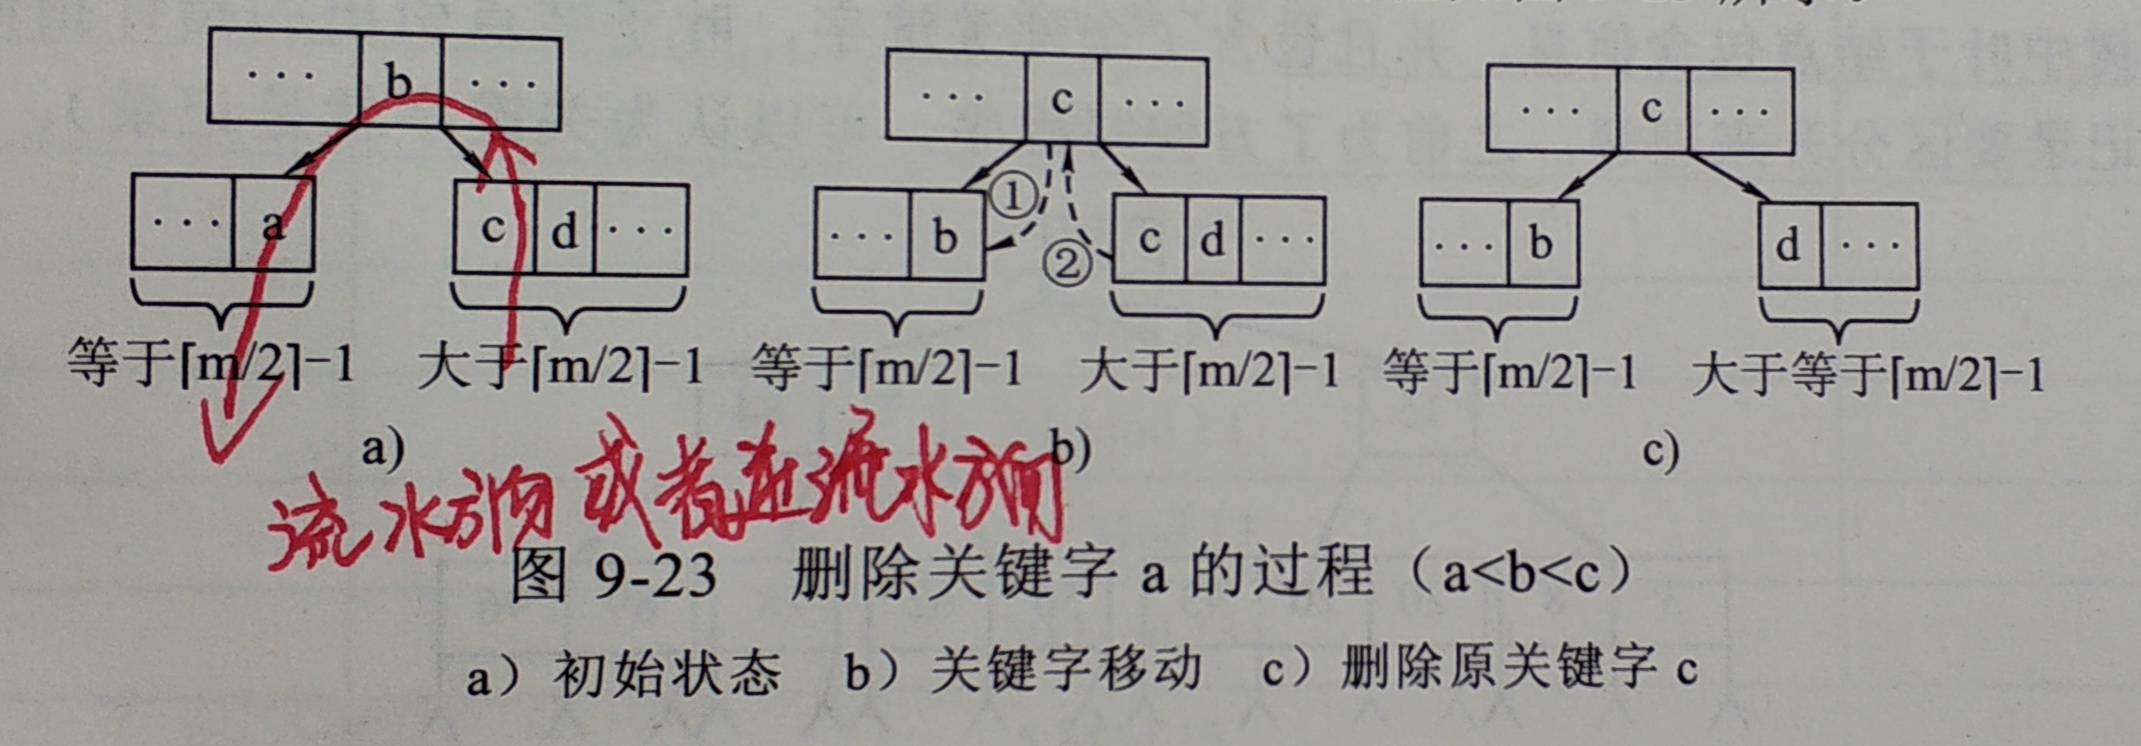
\includegraphics[scale=0.1]{example/chapter6/IMG_20181127_192544.png}
			\end{figure}

			\item 如果不在终端节点上,要替换替换到终端节点上
			\item 如果左右节点都是最少节点,则要掉下来一个,{\color{red}逆上升过程}

			\begin{figure}[H]
				\centering  % 环境中的内容居中排版
				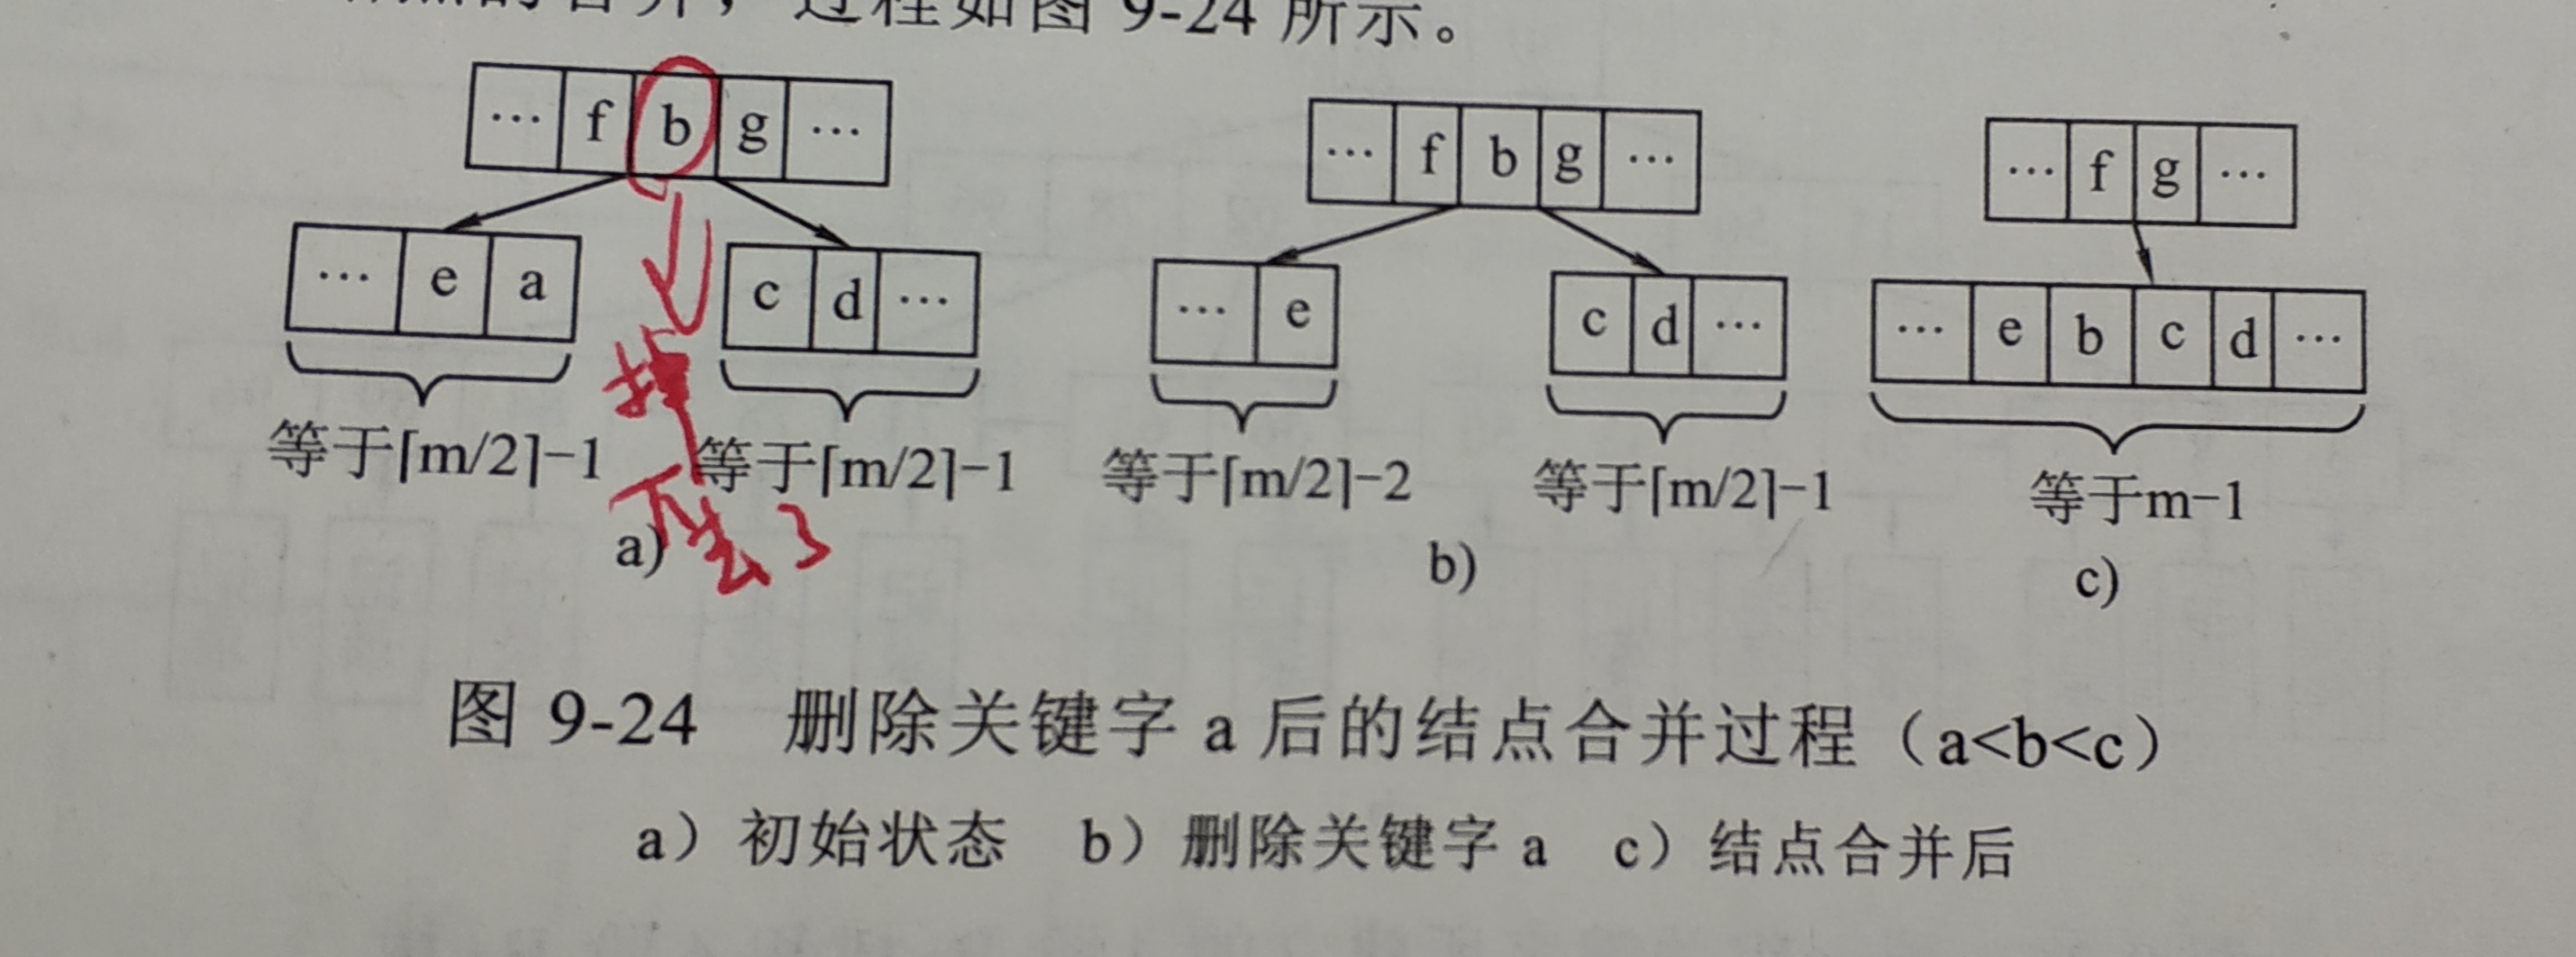
\includegraphics[scale=0.1]{example/chapter6/IMG_20181127_193515.png}
			\end{figure}
	\end{itemize}
\end{itemize}

\section{真题实战}


\subsection{2017年第(4)题}

\begin{lstlisting}[basicstyle=\small\ttfamily, caption={}, numbers=none]
对下面的3阶B-树,一次执行下列操作,画出各步操作的结果
1)插入90 2)插入25 3)插入45  4)删除60  5)删除80
\end{lstlisting}
\begin{figure}[H]
	\centering  % 环境中的内容居中排版
	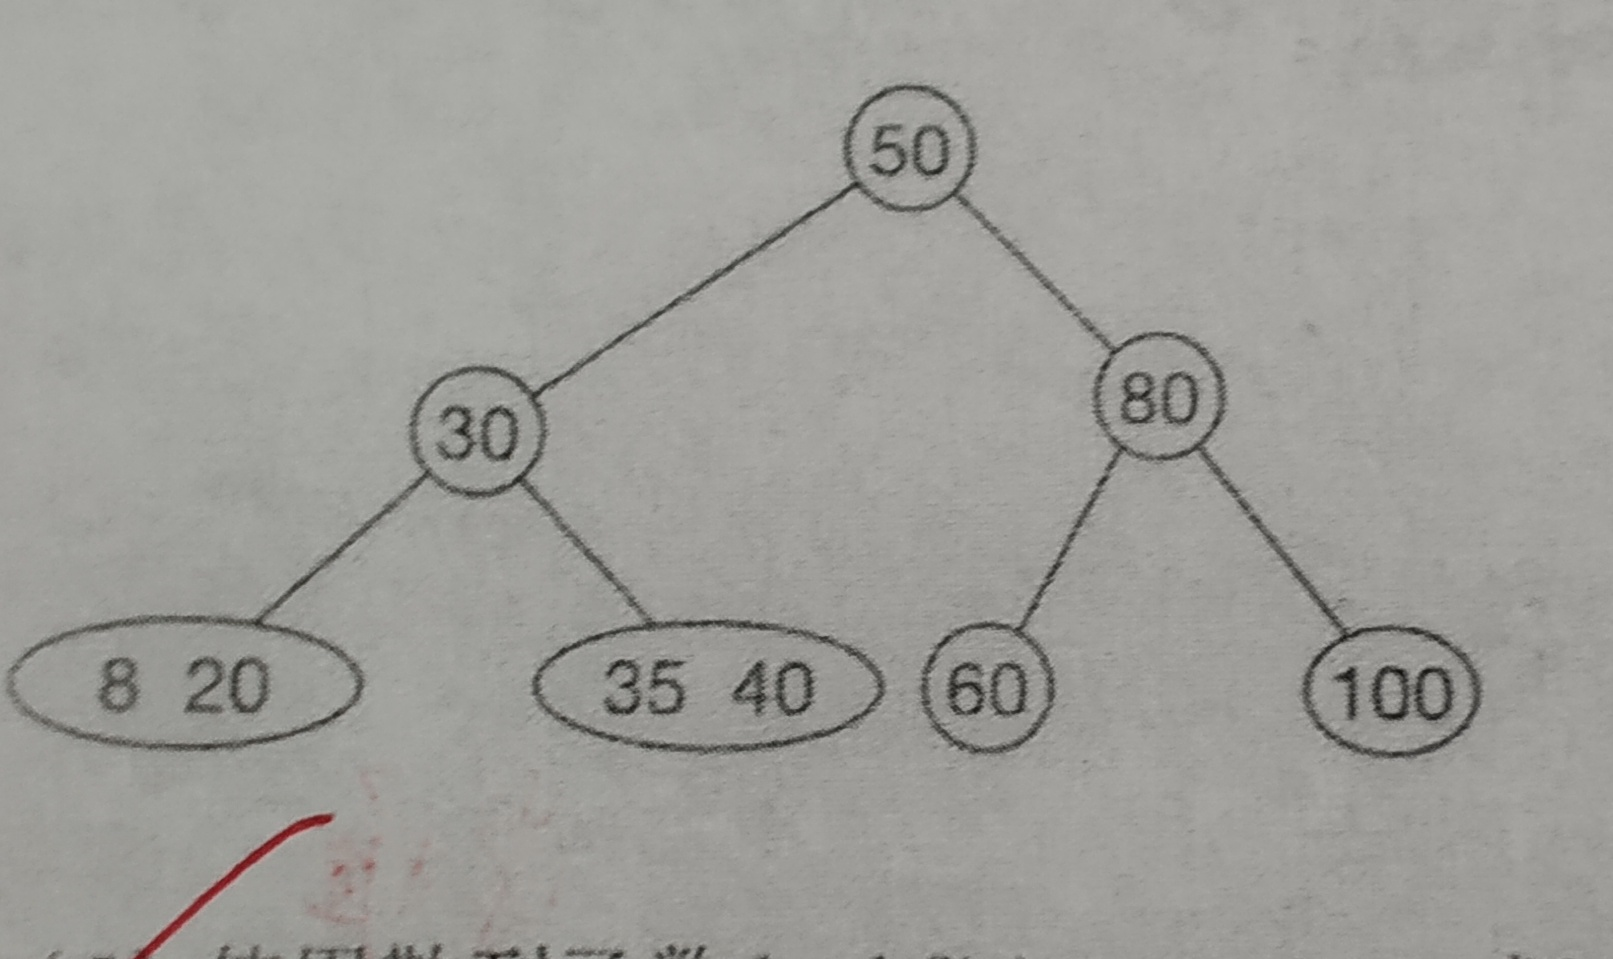
\includegraphics[scale=0.1]{example/chapter6/IMG_20181127_173638.png}
\end{figure}
解:\newline
\begin{figure}[H]
	\centering  % 环境中的内容居中排版
	\includegraphics[scale=0.1]{example/chapter6/IMG_20181127_200414.png}
\end{figure}


\subsection{2015年第(3)题}

\begin{figure}[H]
	\centering  % 环境中的内容居中排版
	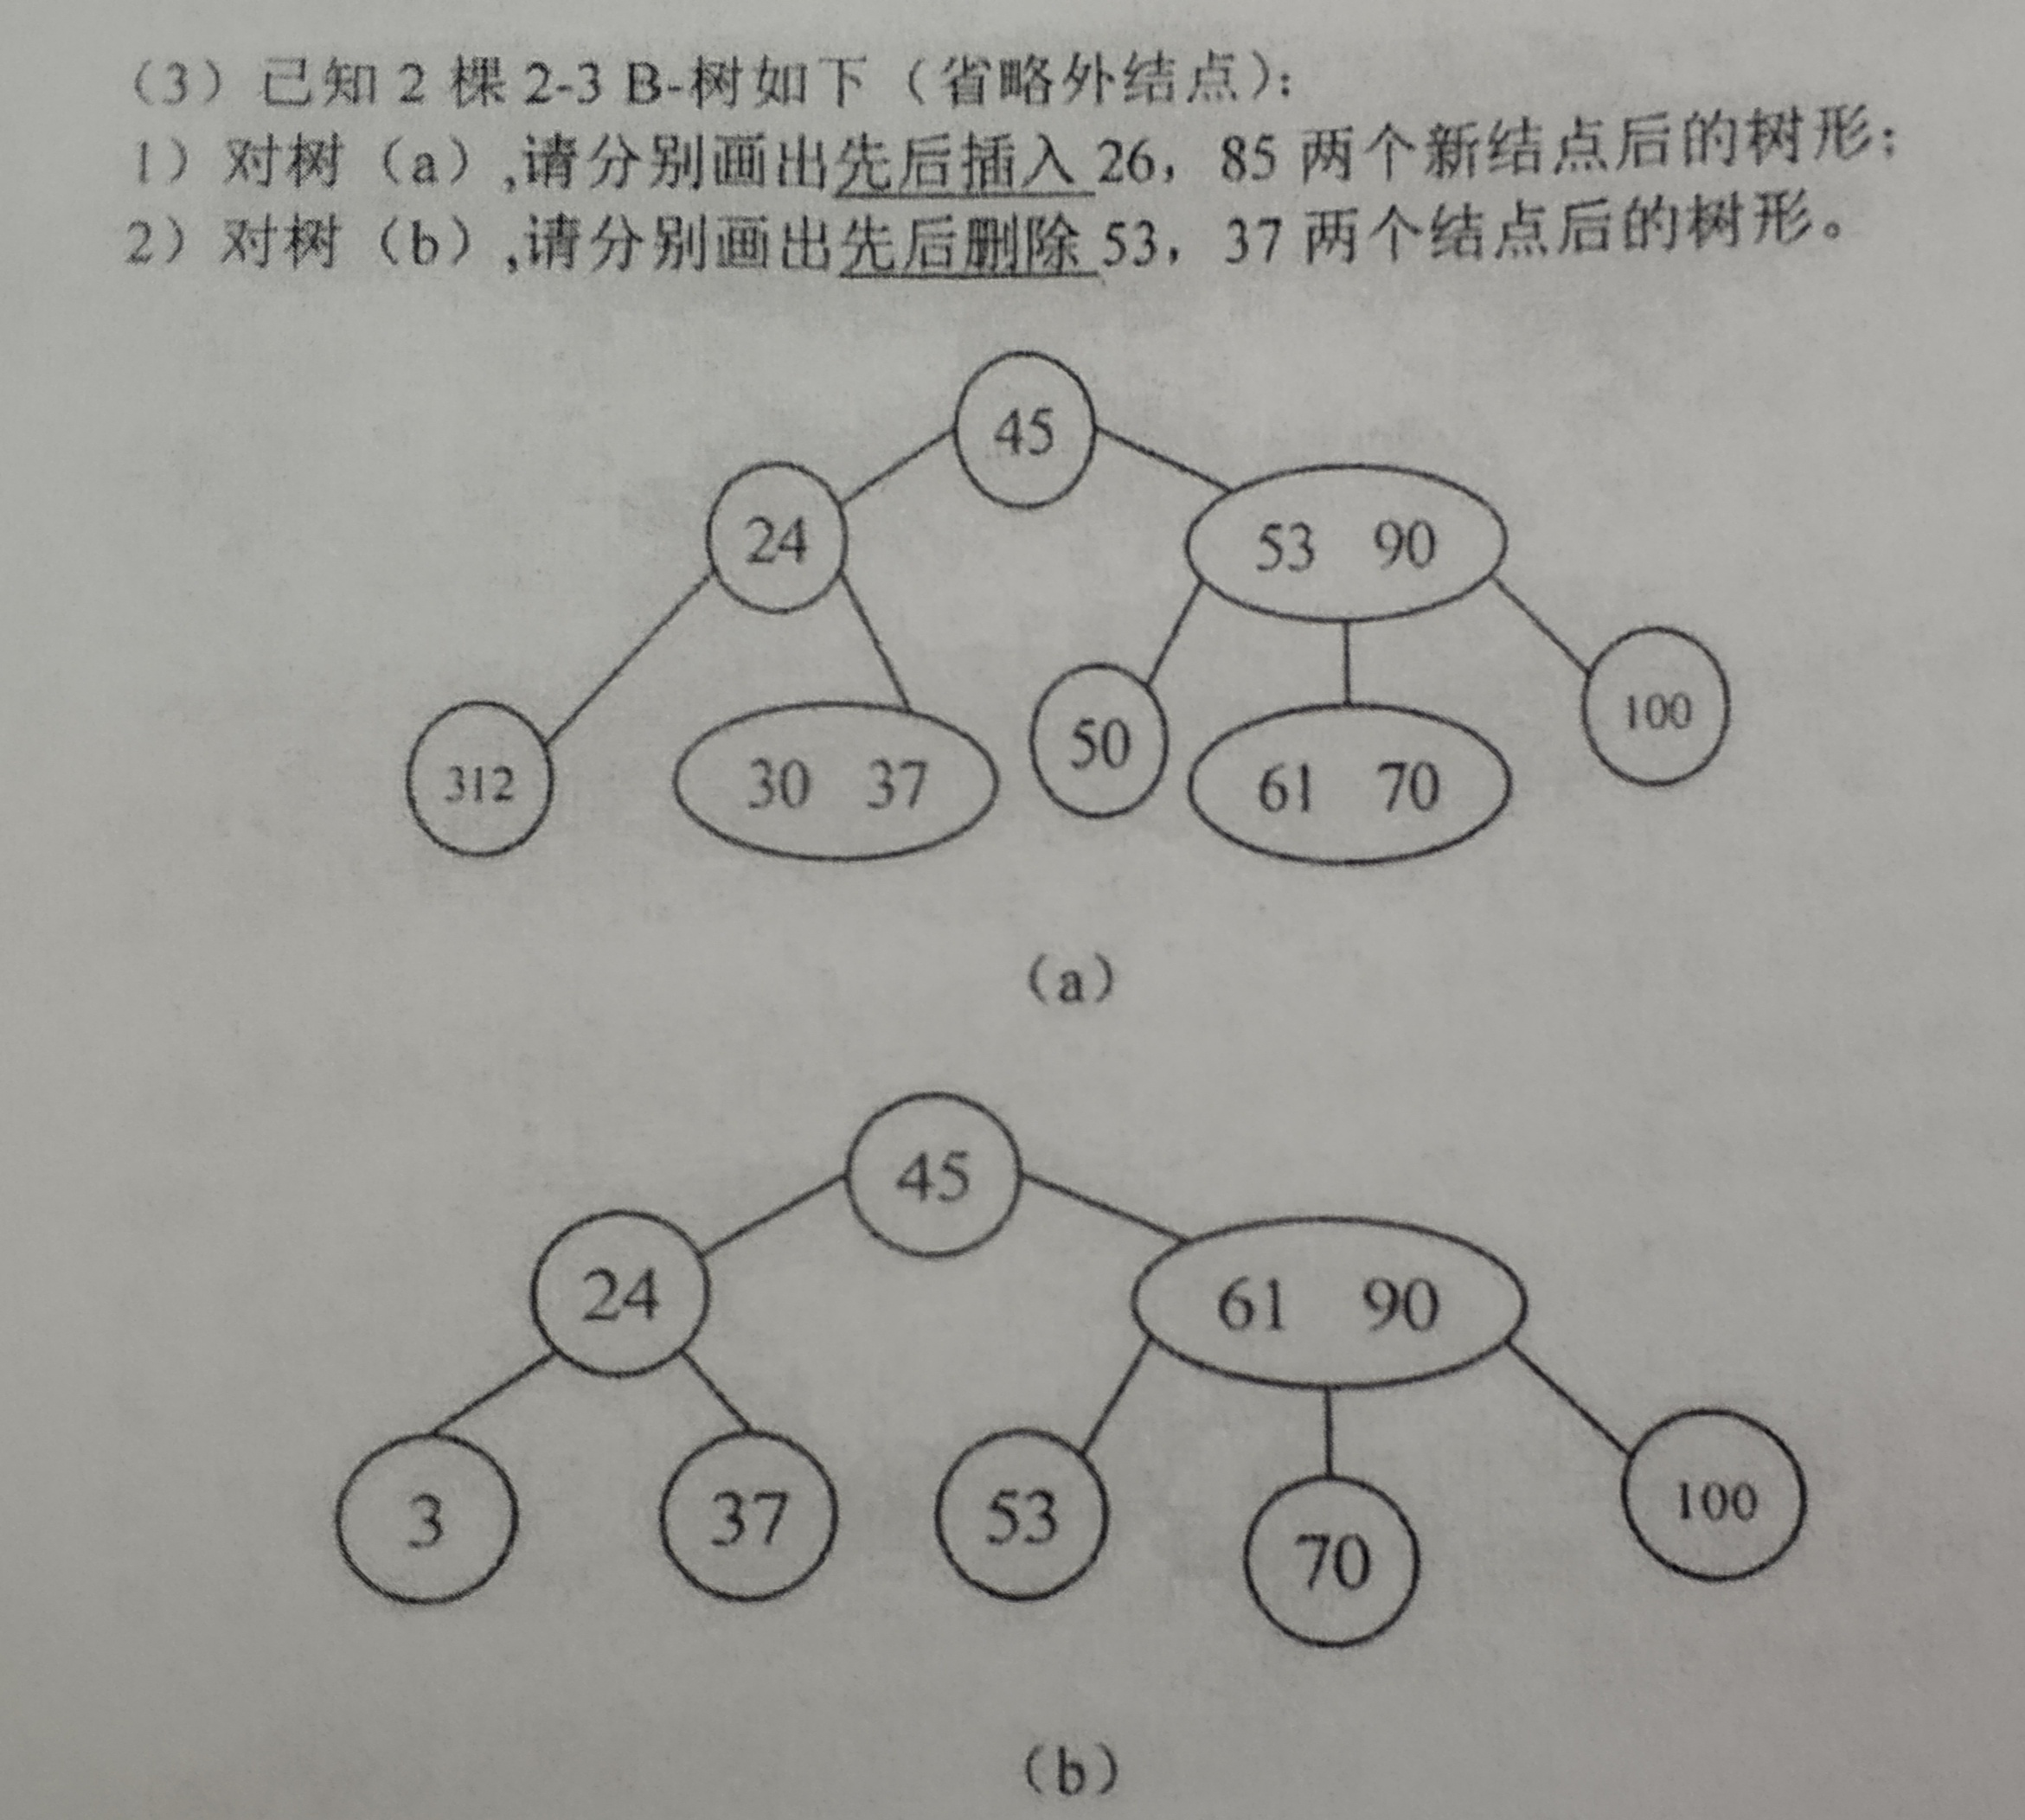
\includegraphics[scale=0.1]{example/chapter6/IMG_20181127_200601.png}
\end{figure}

解:\newline
\begin{figure}[H]
	\centering  % 环境中的内容居中排版
	\includegraphics[scale=0.1]{example/chapter6/IMG_20181127_202059.png}
\end{figure}

\subsection{2012年408}
已知一棵3阶B树,如下图所示。删除关键字78得到一棵新B树,其最右节点中的关键字是(  ).\newline
\begin{figure}[H]
	\centering  % 环境中的内容居中排版
	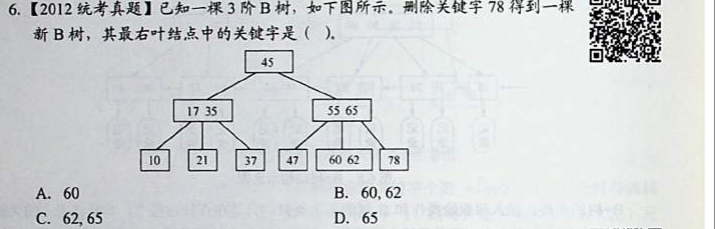
\includegraphics[scale=0.1]{example/chapter6/Annotation2019-09-25182756.png}
\end{figure}
解:\newline
B-树也满足一定的排序树的性质,一定要把握这一点。然后左边的节点足够借,然后就会像水流那样流动数据.\newline
\begin{figure}[H]
	\centering  % 环境中的内容居中排版
	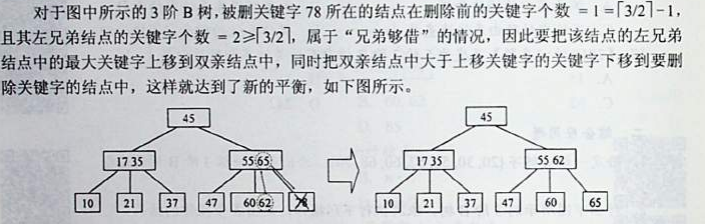
\includegraphics[scale=0.3]{example/chapter6/Annotation2019-09-25183110.png}
\end{figure}

\subsection{王道简单题}
高度为5的3阶B树至少有(  )个结点,至多有(   )个结点。\newline
A. 32 B . 31 C.120 D. 121\newline
解:\newline
问结点数而不是关键字树。\newline
至少就相当于一棵满二叉树,$2^5 - 1 = 31$ 个结点。\newline
至多就相当于一棵满三叉树,$3^5 - 1 = 121$个结点。\newline
